\documentclass[11pt]{article}
\usepackage[margin=1in]{geometry}
\usepackage{graphicx}
\usepackage{amsmath}
\usepackage{booktabs}
\usepackage{subcaption}
\usepackage[hidelinks]{hyperref}

\graphicspath{{figures/}}
\newcommand{\xunit}{\ensuremath{10^{-38}~\mathrm{cm^2/Ar}}}

\title{MicroBooNE NuMI FHC charged-current \boldmath$1\mu\,1\pi^{\pm}\,Xp$\\
       differential cross sections: the XSecAnalyzer framework}
\author{Framework-only summary note}
\date{\today}

\begin{document}
\maketitle

\noindent
This note documents the \emph{XSecAnalyzer} framework extraction of the
MicroBooNE NuMI FHC charged-current $\nu_\mu$ $1\mu\,1\pi^{\pm}\,Xp$ differential
cross section. It describes the inputs, the method, and the results of the
framework pipeline alone; the parallel custom-macro pipeline and the
cross-pipeline comparison are documented elsewhere.

\section{Inputs}
\label{sec:inputs}

The measurement uses the MicroBooNE \textbf{Run~1 NuMI FHC} samples. The beam-on
data slot is filled with \textbf{NuWro fake data} for a generator-closure test
(beam-on data is disabled). The simulated samples are:
\begin{itemize}
  \item GENIE $\nu_\mu$ overlay (\texttt{numuMC}), which defines the detector
        response (smearing) and efficiency;
  \item beam-off (EXT) data for the cosmic background;
  \item the dirt (out-of-cryostat) sample;
  \item eight detector-variation samples for the detector systematic uncertainty.
\end{itemize}
Normalisations: data POT $3.283\times10^{20}$; the simulation is scaled by
$0.14101$ (run POT / summed MC POT); the NuWro fake-data slot corresponds to
$6.65042\times10^{20}$~POT. The NuMI $\nu_\mu+\bar\nu_\mu$ flux is integrated to
$\Phi = 2.372512\times10^{-9}~\mathrm{cm^{-2}\,POT^{-1}}$, and the argon target
count is taken over the fiducial volume with the $z$ dead region
($675.1$--$775.1$~cm) excluded. The configuration is driven by
\texttt{file\_properties\_numi.txt}, the per-observable
\texttt{ccpi\_<obs>\_bin\_config.txt}, \texttt{ccpi\_xsec\_config\_numi.txt}, and
\texttt{ccpi\_systcalc\_numi.conf}.

\section{Method}
\label{sec:method}

\paragraph{Signal definition.}
A signal event is a charged-current $\nu_\mu$ interaction with a true vertex in
the fiducial volume, exactly one muon and exactly one charged pion, any number of
protons ($Xp$, $X\ge0$), and no other mesons. The cross section is reported in
the \textbf{measured phase space}
\begin{equation}
  p_\mu > 0.15~\mathrm{GeV}/c,\qquad
  p_\pi > 0.175~\mathrm{GeV}/c,\qquad
  \theta_{\mu\pi} < 2.6~\mathrm{rad},
\end{equation}
which removes the low-momentum and large-opening-angle regions where the
selection has little acceptance.

\paragraph{Selection.}
The \texttt{CC1mu1piXp} selection requires a reconstructed neutrino vertex in the
fiducial volume with topological score $>0.67$ and at least two tracks; it
identifies the muon candidate as the longest qualifying track (muon PID) and the
pion candidate as the highest-LLR qualifying track, applies track-containment,
gap, and shower-veto requirements, the opening-angle cut $\theta_{\mu\pi}<2.6$,
and an upper track-multiplicity bound. The muon momentum is reconstructed from
multiple Coulomb scattering (\texttt{candidate\_muon\_mom\_mcs}) and the pion
momentum from the proton-hypothesis range.

\paragraph{Extraction chain.}
The processed ntuples are produced by \texttt{ProcessNTuples}; \texttt{univmake}
then builds the response matrix, backgrounds, and the full set of systematic
universes per observable; and \texttt{Unfolder} performs a \textbf{Wiener--SVD}
unfolding (second-derivative regularisation) using the full
systematic-plus-statistical covariance. The cross section in each true bin is
obtained from the unfolded signal $N$ via the conversion factor,
\begin{equation}
  \sigma = \frac{N}{N_{\mathrm{Ar}}\,\Phi},
\end{equation}
with $N_{\mathrm{Ar}}$ the in-FV argon target count. The systematic budget
includes the flux (PPFX), GENIE cross-section (UBGenie and unisim/reweight),
detector variations, hadron reinteraction, dirt normalisation, finite MC/EXT
statistics, and POT.

\paragraph{Validation.}
The framework passes the NuWro fake-data closure test: unfolding the NuWro
pseudo-data through the GENIE-built response recovers the input generator truth
within the quoted statistical precision, confirming that the response,
background subtraction, and unfolding are internally consistent.

\section{Results}
\label{sec:results}

Table~\ref{tab:integrated} lists the integrated cross section obtained for each
observable in the measured phase space, and Fig.~\ref{fig:diff} shows the
corresponding differential distributions with their full (systematic plus
statistical) uncertainty bands.

\begin{table}[htbp]
  \centering
  \caption{Integrated framework cross section per observable (measured phase
           space), in units of \xunit.}
  \label{tab:integrated}
  \begin{tabular}{lc}
    \toprule
    Observable & $\sigma$ [\xunit] \\
    \midrule
    $p_\mu$            & 0.442 \\
    $p_\pi$            & 0.531 \\
    $\cos\theta_\mu$   & 0.559 \\
    $\cos\theta_\pi$   & 0.450 \\
    $\theta_{\mu\pi}$  & 0.444 \\
    \bottomrule
  \end{tabular}
\end{table}

\begin{figure}[htbp]
  \centering
  \begin{subfigure}{0.48\textwidth}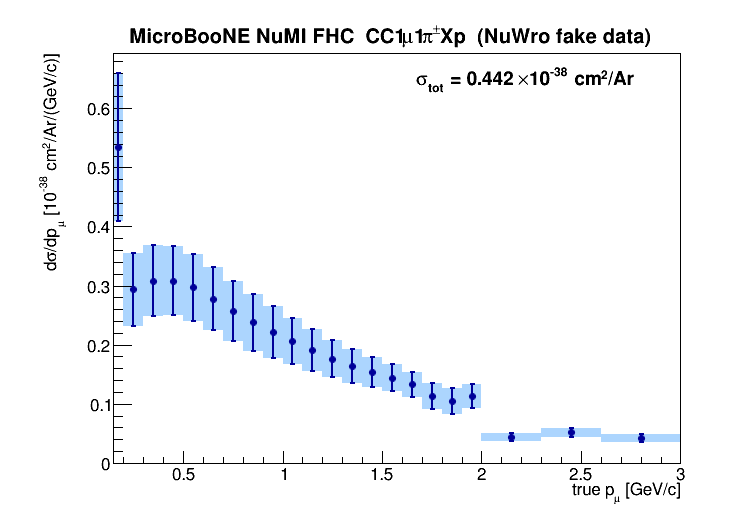
\includegraphics[width=\linewidth]{fw_xsec_pmu.png}\caption{$p_\mu$}\end{subfigure}\hfill
  \begin{subfigure}{0.48\textwidth}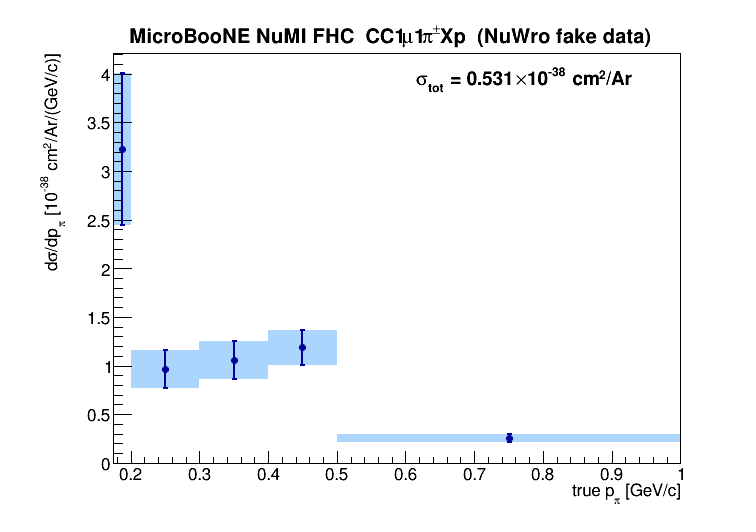
\includegraphics[width=\linewidth]{fw_xsec_ppi.png}\caption{$p_\pi$}\end{subfigure}

  \begin{subfigure}{0.48\textwidth}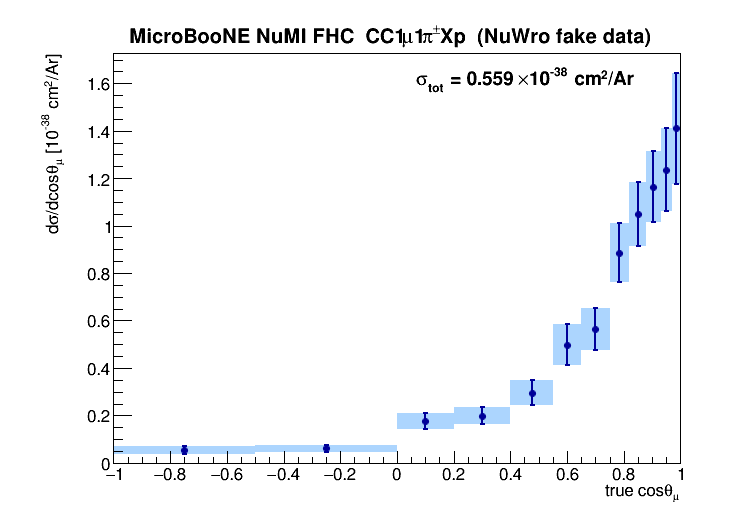
\includegraphics[width=\linewidth]{fw_xsec_costhmu.png}\caption{$\cos\theta_\mu$}\end{subfigure}\hfill
  \begin{subfigure}{0.48\textwidth}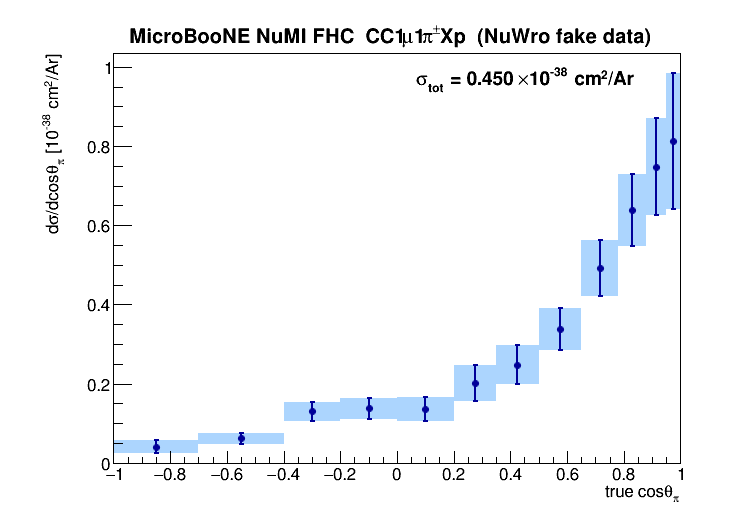
\includegraphics[width=\linewidth]{fw_xsec_costhpi.png}\caption{$\cos\theta_\pi$}\end{subfigure}

  \begin{subfigure}{0.48\textwidth}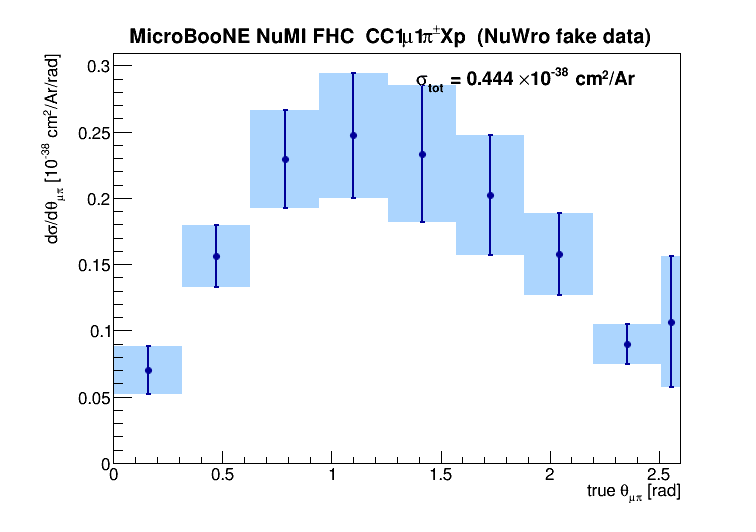
\includegraphics[width=\linewidth]{fw_xsec_thmupi.png}\caption{$\theta_{\mu\pi}$}\end{subfigure}
  \caption{Framework Wiener--SVD unfolded differential cross sections
    $d\sigma/dx$ (NuWro fake data) in the measured phase space. Points are the
    unfolded result; the shaded band is the full systematic-plus-statistical
    uncertainty. The first $p_\mu$/$p_\pi$ bins and the last $\theta_{\mu\pi}$
    bin are narrow because they are truncated at the phase-space boundaries.}
  \label{fig:diff}
\end{figure}

\end{document}
